%
% File ACL2016.tex
%

\documentclass[11pt]{article}
\usepackage{acl2016}
\usepackage{times}
\usepackage{latexsym}
\usepackage{algorithmic}
\usepackage{graphicx}

%\aclfinalcopy % Uncomment this line for the final submission
%\def\aclpaperid{***} %  Enter the acl Paper ID here

% To expand the titlebox for more authors, uncomment
% below and set accordingly.
% \addtolength\titlebox{.5in}    

\newcommand\BibTeX{B{\sc ib}\TeX}


\title{Fast, Scalable Phrase-Based SMT Decoding}

% Author information can be set in various styles:
% For several authors from the same institution:
% \author{Author 1 \and ... \and Author n \\
%         Address line \\ ... \\ Address line}
% if the names do not fit well on one line use
%         Author 1 \\ {\bf Author 2} \\ ... \\ {\bf Author n} \\
% For authors from different institutions:
% \author{Author 1 \\ Address line \\  ... \\ Address line
%         \And  ... \And
%         Author n \\ Address line \\ ... \\ Address line}
% To start a seperate ``row'' of authors use \AND, as in
% \author{Author 1 \\ Address line \\  ... \\ Address line
%         \AND
%         Author 2 \\ Address line \\ ... \\ Address line \And
%         Author 3 \\ Address line \\ ... \\ Address line}
% If the title and author information does not fit in the area allocated,
% place \setlength\titlebox{<new height>} right after
% at the top, where <new height> can be something larger than 2.25in
\author{Hieu Hoang\\
	    Moses Machine Translation CIC\\
	    {\tt hieu@moses-mt.org}
	  \And
	Author 2\\
  	ABC University\\
  	900 Main Street\\
  	Ourcity, PQ, Canada A1A 1T2\\
  {\tt author2@abc.ca}}

\date{}

\begin{document}

\maketitle

\begin{abstract}
The utilization of statistical machine translation (SMT) has grown enormously over the last decade, many using open-source software developed by the NLP community. As commercial utilization has increased, there has been a pressing need that is optimized for their requirements. Specifically, faster phrase-based decoding, and more efficient utilization of modern multicore servers.

We present in this paper a re-assessment of the major components of phrase-based decoding and decoder implementation with particular emphasis on speed and scalability to multicore machines. The result is a drop-in replacement for the Moses decoder which is up to fifteen times faster and scales almost linearly with the number of cores. Furthermore, the decoder makes less search errors than the current Moses decoder.

\end{abstract}

\section{Introduction}

SMT has been one of the outstanding success story from the NLP community in the last decade, progressing from a mostly research discipline to public useability via services such as Google Translate, Microsoft Translator Hub, as well as services and products built around offline products such as Language Weaver and the open-source Moses toolkit. The latter has spawned a cottage industry  encompassing a range of organizations and services from small language service providers seeking to reduce translation cost, to large inter-govermental organizations such as the EU and the UN that require high volume, high quality translation.

For high volume users, decoding is a largest and most critical part of the translation process which needs to be fast and efficient. However, it has been noticed that the Moses decoder, amongst others, is unable to efficiently use multiple CPU cores that are now common on modern servers (reviewed paper, github discussion). That is, the time taken to decode a test set does not substantial decrease when more cores are used, in fact, decoding time may increase when more cores are added. The problem will continue to grow as the commercial use of SMT increases and the number of CPU cores increases.

There have be speculation on the causes of the inefficiency as well as potential remedies. This paper is the first we know of that seeks to tackle this problem head on. We present an phrase-based decoder that is not only significantly faster than the Moses baseline for single-threaded operation, but is able to scale run multiple threads on multicore machines with only a slightly loss in linear speed. Model scores and functionality are compatible with Moses to aid comparison and ease of transition for users. All source code will be made available under an open-source license.

\subsection{Prior Work}

There are a number of open-source SMT projects, most includes a decoder. The most well known is Moses, which supports phrase-based models, hierarchical phrase-based as well as various syntax-based models. Joshua also supports hiearchical and syntax models and has recently supported phrase-based models. Phrasal supports a number of variants of the phrase-based model. CDEC supports hierarchical and syntactic models.

A number of the decoders support multithreading whilst others use alternative methods such as Hadoop or external scripts to parallelize decoding. We shall investigate the efficiency of using parallelizing decoding using the multi-processor approach. None of the decoder focus on multi-threads decoding. 

(Recently reviewed) describes running multiple processes of the Moses decoder for increased speed.

Other prior work look to optimizing specific components of decoding. (Liang and Chiang) describes the cube-pruning and cube-growing algorithm for decoding which allows the tradeoff between speed and translation quality to the adjusted with a simgle parameter. (KenLM) and (DALM) describes fast, efficient datastructures for language models. (Zen) describes an implementation of a phrase-table for an SMT decoder that is loaded on demand, reducing the initial loading time and memory requirements. (CompactPT) extends this by compressing the on-disk phrase table and lexicalized re-ordering model resulting in impressive speed gains over previous work.

(mtplz) is perhaps closest in intent to this work. This takes a wholistic approach to decoding, describing a novel decoding algorithm which is fis focused on better decoding speed. It also describes a number of implementation details for faster decoding. However, the decoding algorithm is only able to incorporate one stateful feature function which precludes some of the useful decoding configurations which contains multiple stateful feature functions. It does not include a load-on-demand phrase table, therefore, cannot be used in a commercial environment where phrase-table has not be filtered with a know test set for any realistic size phrase-table. Neither did this paper analyze the scalability of their work to multicore servers.

The rest of the paper will be broken up into the following sections. Next, we will describe the phrase-based model and the major implementation components, with particular emphasis on decoding time shortcomings. We will then describe modifications to improve decoding speed and present results. We conclude in the last section discuss suggested improvements and future work.

\section{Phrase-Based Model}

The objective of decoding is to find the target translation with the maximum probability, given a source sentence. That is, for a source sentence $s$, the objective is to find a target translation $\hat{t}$ which has the highest conditional probability $p(t | s)$. Mathematically, this is written as:
\begin{equation}
\hat{t} = \arg \max_t p( t | s )
\label{eq:argmax-factored-trans}
\end{equation}
where the \emph{arg max} function is the search. The log-linear model generalizes Equation~\ref{eq:argmax-factored-trans} to include more component models and weighting each model according to the contribution of each model to the total probability. 
\begin{equation}
\label{eq:Log-Linear}
p(t | s) 	=  \frac{1}{Z} \exp ( \sum_m \lambda_m h_m ( t, s)^{} )
\end{equation}
where $\lambda_m$ is the weight, and $h_m$ is the feature function, or `score', for model $m$. $Z$ is the partition function which can be ignored for optimization. 

\subsection{Beam Search}

A translation of a source sentence is created by applying a series of translation rules which together translate each source word once, and only once. Each partial translation is called a \emph{hypothesis}, which is created by applying a rule to an existing hypothesis. This process is called \emph{hypothesis expansion} and starts with a hypothesis that has translated no source word and ends with a completed hypothesis that has translated all source words. The highest-scoring completed hypothesis, according to the model score, is returned as  most probable translation, $\hat{t} $. Incomplete hypotheses are referred to as partial hypotheses.

Each rule translates a contiguous sequence of source words but successive translation options do not have to be adjacent on the source side, depending on the distortion limit. However, the target output is constructed strictly left-to-right from the target string of successive translation options. Therefore, successive translation options which are not adjacent and monotonic in the source causes translation reordering.

A beam search algorithm is used to create the completed hypothesis set efficiently. Partial hypotheses are organized into stacks where each stack holds a number of comparable hypotheses. Hypotheses in the same stack have the same coverage cardinality $|C|$, where $C$ is  the coverage set, $C \subseteq \{1,2,... |s| \} $ of the number of  source words translated. Therefore, $|s| + 1$ number of stacks are created for the decoding of a sentence $s$. 

There are three main optimization to the search that we shall investigate. Firstly, the search creates and destroy a large number of hypothesis objects in memory which puts a heavy burden on the operating system. We shall optimize the search algorithm to use memory pools and object pools, replacing the operating system's general purpose memory management with our own application-aware management. 

The speed of memory access is dependent on whether the data is in the CPU cache which is a constrained resource compared to memory size, typically 20MB in the latest processors. We shall seek to re-use recently accessed information to increase likelihood of the data being in the CPU cache. 

In multiprocessor servers, the CPU cache is attached to each processor and each core. If a sentences is being decoded on one CPU is switched to another, the CPU cache on the new CPU must be repopulated, slowing down decoding. We will therefore investigate binding threads to specific cores.

Lastly, we shall investigate different stack configurations other than coverage cardinality to see whether they can improve speed and translation quality.

\subsection{Feature Functions}

Features functions are the $h_m$ in Equation~\ref{eq:Log-Linear}, calculating a score for each hypothesis.

The standard feature functions in the phrase-based model include:
\begin{enumerate}
  \item log transforms translation model probabilities, $p_{TM}(t|s) $ and $p_{TM}(s|t)$, and word-based translation probabilities $p_w(t|s)$ and $p_w(s|t)$,
  \item log transforms of the lexicalized re-ordering probabilities,
  \item log transforms of the target language model probability $p(t)$, 
  \item a distortion penalty
  \item a phrase-penalty,
  \item a word penalty,
  \item an unknown word penalty.
\end{enumerate}
%which we have suffixed with $_{TM} $ to avoid confusion with the overall model probability $ p(t|s) $ and $ p(s|t)$. 

The first three feature functions frequently trained on data and require the feature to read the model from files. The other feature functions do not require model files. We shall investigate the first two feature functions for optimization.

%\subsection{Language Model}
% TODO
%
\subsection{Translation Model}

Load-on-demand \emph{'binary'} phrase-tables are often used for MT deployment due to their fast loading and querying speed, and because they can be used with large phrase-tables. We therefore focus on optimizing decoding speed with these phrase-tables, specifically the Probing PT.

We shall look at the caching strategies to reduce the number of phrase-table lookups. We shall also investigate the datastructures used by the phrase-table and their impact on decoding speed.

\subsection{Lexicalized Reordering Model}

The lexicalized reordering model is trained on parallel data, usually requiring random lookups of the model file during decoding. However, the key to the lookup are the source and target phrase of each translation rule. We shall investigate the advantages of storing the mode data within the translation rule.

\section{Experimental Setup}

We trained a phrase-based system using the Moses toolkit with standard settings. The training data consisted of most of the publicly available Arabic-English data from Opus (Jörg Tiedemann, 2012,) containing over 69 million parallel sentences, and tuned on a held out set. The phrase-table was then pruned, keeping only the top 100 entries per source phrase, according to $p(t|s)$. All models files were then binarized; the language models were binaized using KenLM (???), the phrase table using Probing PT (???), lexicalized reordering model using the compact datastructure described in ???. These binary formats were choosen for their best-in-class multithreaded performance. Table~\ref{tab:model-files} gives details of the resultant sizes of the model files. For verification with a different dataset, we also occasionally used a second system trained on the French-English Europarl corpus (2m parallel sentences). 
\begin{table}[h]
\begin{center}
\begin{tabular}{|l|c|c|} \hline
		& ar-en	& fr-en \\ \hline
Phrase table  	& 17 	& 5.8 \\
Language model 	& 3.1  	& 1.8 \\ 
Lex-re model	& 2.3	& 637MB \\ \hline
\end{tabular}
\end{center}
\caption{Model sizes in GB}
\label{tab:model-files}
\end{table}
For testing decoding speed, we used a subset of the training data, Table~\ref{tab:test-sets}. The two test scenarios have differing characterics that we are interested in analyzing, ar-en have short sentences with large models while fr-en have overly long sentences with smaller models.

\begin{table}[h]
\begin{center}
\begin{tabular}{|l|c|c|} \hline
		& ar-en	& fr-en \\ \hline
\# sentences  	& 800k 	& 200k \\
\# words 	& 5.8m 	& 5.9m \\ 
Avg words/sent	& 7.3	& 29.7 \\ \hline
\end{tabular}
\end{center}
\caption{Test sets}
\label{tab:test-sets}
\end{table}

Where we need to compare model scores, we used held out test sets; a 2,000 sentence subset of OpenSubtitles for ar-en and the 3,003 sentence newstest2011 test set for fr-en.

Standard Moses phrase-based configurations are used, except that we use the cube-pruning algorithm (???) with a pop-limit of 400, rather than the basic phrase-based algorithm. The cube-pruning algorithm is often employ by users who require fast decoding as it gives them the ability to trade speed with translation quality with a simple pop-limit parameter.

As a baseline, we use the latest version of the Moses decoder taken from the github repository.

For all experiments, we used a Dell PowerEdge R620 server with 16 cores, 32 hyper-threads, split over 2 physical processors (Intel Xeon E5-2650 @ 2.00GHz). The server has 380GB RAM. The operating system was Ubuntu 14.04, the code was compiled with gcc 4.8.4 and Boost library 1.59.

\section{Results}

\subsection{Optimizing Memory}

We create a dynamic memory pool which can grow as more memory is requested. The memory is not released, instead the pool can be reset in order for the memory to be re-used. We instantiate two pools for each thread, one which is never reset and another which is reset after the decoding each sentence. Objects are created in either pool according to their life cycle.

For critical objects with high churn such as the hypotheses, thread-specific LIFO queues are used to recycle objects which are no longer used. This not only reduces memory wastage but re-uses recent objects which are likely to be in the CPU cache.

Over 24\% of the Moses decoder running time is spent on memory management and this increases when more threads are used, Table~\ref{tab:optimizing-memory}, dampening the scalability ofthe decoder. By contrast, our decoder spends 11\% on memory management and does not significantly increase with more cores.
\begin{table}[h]
\begin{center}
\begin{tabular}{|l|c|c|c|c|} \hline
		& \multicolumn{2}{c|} {Moses}	& \multicolumn{2}{c|} {Our Work} \\ \hline
\# threads	& 1 		& 32	& 1 		& 32  \\ \hline
Memory  	& 24		& 39 	& 11		& 13 \\
LM 		& 12	 	& 2 	& 47		& 38 \\ 
Phrase-table	& 9	 	& 5 	& 2		& 4 \\ 
Lex RO 		& 8	 	& 2 	& 2		& 2 \\ 
Search 		& 2	 	& 0 	& 14		& 19 \\ 
Misc/Unknown	& 45	 	& 39 	& 24		& 29 \\ \hline
\end{tabular}
\end{center}
\caption{Profile of \%age decoding time}
\label{tab:optimizing-memory}
\end{table}

% A potential disadvantage of using memory pool is that the decoder will use more memory, however, Table~\ref{tab:memory-usage} shows that peak memory consumption are comparable.
% \begin{table}[h]
% \begin{center}
% \begin{tabular}{|l|c|c|} \hline
% 		& 1 thread	& 32 threads \\ \hline
% Moses  		& ???	 	& ??? \\
% Our work 	& ??? 		& ??? \\ \hline
% \end{tabular}
% \end{center}
% \caption{Peak Memory Usage in GB}
% \label{tab:memory-usage}
% \end{table}

\subsection{Stack Configuration}

The most popular stack configuration for phrase-based model, as implemented in Pharaoh, Moses and Joshua, has been by coverage cardinality, ie. hypotheses that have translated the same number of source words are stored in the same stack. There have been research into other stack layouts such as~\cite{ortizmartinez-garciavarea-casacuberta:2006:WMT}, and it has been noted that the decoder in~\cite{Brown:1993} uses coverage stacks, as opposed to coverage cardinality. 

We also note that distortion limit which constrains hypothesis extension is dependent on the hypothesis' coverage vector, $C$ \emph{and} the end position of most recent source word that has been translated, $e$. The distortion limit must be checked for every instance of a hypothesis and translation rule, Figure~\ref{algo:Hypothesis Expansion with Unsorted Stack}.
\begin{figure} [h]
\begin{algorithmic}
%\REQUIRE source sentence $s$, translation options
\FORALL{ $hypo$ in $stack_{|C|}$} 
  \FORALL{ translation rules}
      \IF {can-expand($C(hypo)$, $e(hypo)$, translation rule range)}
	\STATE expand hypo with translation rule $\rightarrow$ new hypo
	\STATE add new hypo to next stack
      \ENDIF
  \ENDFOR % { translation options}
\ENDFOR % { hypothesis in $stack_i$} 
\end{algorithmic}
\caption{Hypothesis Expansion with Unsorted Stack}
\label{algo:Hypothesis Expansion with Unsorted Stack}
\end{figure}
However, by separating hypotheses into \emph{'ministacks'} according to coverage and end position, the distortion limit only needs to be checked for each ministack, Figure~\ref{algo:Hypothesis Expansion with Sorted Stack}.
\begin{figure} [h]
\begin{algorithmic}
%\REQUIRE source sentence $s$, translation options
\FORALL{ $ministack_{C, e}$ in $stack_{|C|}$} 
  \FORALL{ translation rules}
    \IF {can-expand($C$, $e$, translation rule range)}
      \FORALL{ $hypo$ in $ministack_{C, e}$} 
	\STATE expand hypo with translation rule $\rightarrow$ new hypo
	\STATE add new hypo to next ministack
      \ENDFOR
    \ENDIF
  \ENDFOR % { translation options}
\ENDFOR % { hypothesis in $stack_i$} 
\end{algorithmic}
\caption{Hypothesis Expansion with Sorted Stack}
\label{algo:Hypothesis Expansion with Sorted Stack}
\end{figure}
We therefore looked at the effects of three stack configurations.
\begin{enumerate}
  \item coverage cardinality,
  \item coverage,
  \item coverage and end position of most recent translated source word.
\end{enumerate}
We therefore looked at the effects of three stack configurations.
\begin{enumerate}
  \item coverage cardinality,
  \item coverage,
  \item coverage and end position of most recent translated source word.
\end{enumerate}
Table~\ref{tab:stack-configuration} and Figure~\ref{fig:stack-configuration} present the decoding time and average model on the held out test set.
\begin{table}[h]
\tiny
\begin{center}
\begin{tabular}{|r|r|r|r|r|r|r|} \hline
Pop-limit	& \multicolumn{2}{c|}{Cardinality}	& \multicolumn{2}{c|}{Coverage}	& \multicolumn{2}{c|}{Coverage \& end pos} \\ \hline
		& Time		& Score			& Time		& Score		& Time		& Score	\\ \hline
100  		& 73		& -8.64513 		& 75		& -8.64513	& 72	& -8.64513 \\
500		& 237		& -8.59563		& 225		& -8.59563 	& 229	& -8.59612 \\
1,000	 	& 416		& -8.58700		& 397		& -8.58700	& 423	& -8.5870 \\ 
5,000 		& 1930		& -8.58165		& 1931		& -8.58165	& 2153	& -8.58098 \\ 
10,000 		& 3619		& -8.58133		& 3630		& -8.58133	& 4576	& -8.58015 \\ 
15,000 		& 4830		& -8.58130		& 5001		& -8.58130	& 7156	& -8.57999 \\ 
20,000 		& 5849		& -8.58130		& 5916		& -8.58130	& 9583	& -8.57994 \\ \hline
\end{tabular}
\end{center}
\caption{Decoding time (in secs with 32threads) and average model scores for different stack configurations}
\label{tab:stack-configuration}
\end{table}

\begin{figure}[h]
\centering
\begin{tabular}{cc}
{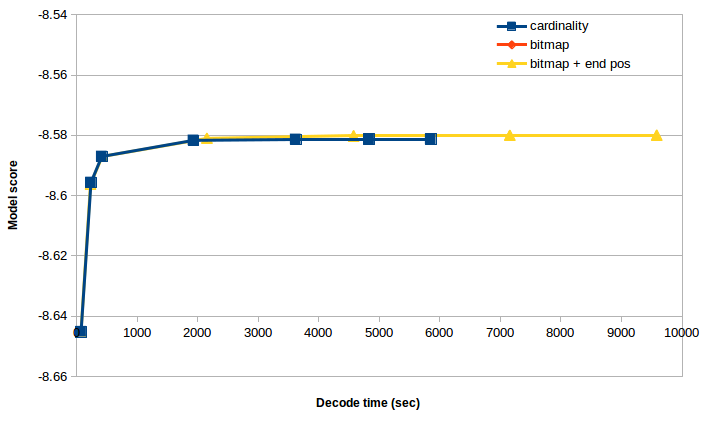
\includegraphics[scale=0.4]{stack-configuration.png}} 
\end{tabular}
\caption{Trade-off between decoding time average model scores for different stack configurations}
\label{fig:stack-configuration}
\end{figure} 

The algorithms in Figure~\ref{algo:Hypothesis Expansion with Unsorted Stack} and ~\ref{algo:Hypothesis Expansion with Sorted Stack} describes the standard phrase-based decoding algorithm, however, the stack configuration issues are the same in the cube-pruning algorithm. Furthermore, the cube-pruning algorithm also contain a priority queue which is attached to coverage cardinality in Moses, Figure~\ref{algo:Cube Pruning with Unsorted Stack}.
\begin{figure} [h]
\begin{algorithmic}
%\REQUIRE source sentence $s$, translation options
\STATE initialize $queue_{|C|}$
\FOR{1 to pop-limit}
  \STATE get best $item$ in $queue_{|C|}$
  \STATE create new hypo from $item$
  \STATE add new hypo to new $stack_{|C|}$
  \STATE create next $items$
  \STATE add new $items$ to $queue_{|C|}$
\ENDFOR % { hypothesis in $stack_i$} 
\end{algorithmic}
\caption{Cube Pruning with Unsorted Stack}
\label{algo:Cube Pruning with Unsorted Stack}
\end{figure}
We experiment with changing the queue, $queue_{|C|}$, by having separate queues for each (1) unique coverage $queue_{C}$, and each (2) unique coverage and end position $queue_{C, e}$. The stack configuration stayed constant.











\section{BLAH BLAH}

The following instructions are directed to authors of papers submitted to and accepted
for publication in the ACL 2016 proceedings.  All authors are required
to adhere to these specifications. Authors are required to provide 
a Portable Document Format (PDF) version of
their papers.  The proceedings will be printed on A4 paper.
Authors from countries where access to word-processing systems is
limited should contact the publication chairs as soon as possible.
 Grayscale readability of all figures and
graphics will be encouraged for all accepted papers
(Section \ref{ssec:accessibility}).  

Submitted and camera-ready formatting is similar,
  however, the submitted paper should have:
\begin{enumerate} 
\item Author-identifying information removed
\item A `ruler' on the left and right margins
\item Page numbers 
\item A confidentiality header.  
\end{enumerate}
In contrast, the camera-ready {\bf should  not have} a ruler, page numbers, nor a confidentiality header.  By uncommenting {\small\verb|\aclfinalcopy|} at the top of this 
 document, it will compile to produce an example of the camera-ready formatting; by leaving it commented out, the document will be anonymized for initial submission.  Authors should place this command after the {\small\verb|\usepackage|} declarations when preparing their camera-ready manuscript with the ACL 2016 style.


\section{General Instructions}

Manuscripts must be in two-column format.  Exceptions to the
two-column format include the title, as well as the 
authors' names and complete
addresses (only in the final version, not in the version submitted for review), 
which must be centered at the top of the first page (see
the guidelines in Subsection~\ref{ssec:first}), and any full-width
figures or tables.  Type single-spaced.  Do not number the pages 
in the camera-ready version.
Start all pages directly under the top margin.  See the guidelines
later regarding formatting the first page.

The maximum length of a manuscript is eight (8) pages for the main
conference, printed single-sided, plus two (2) pages for references
(see Section~\ref{sec:length} for additional information on the
maximum number of pages). 

By uncommenting {\small\verb|\aclfinalcopy|} at the top of this 
 document, it will compile to produce an example of the camera-ready formatting; by leaving it commented out, the document will be anonymized for initial submission.  When you first create your submission on softconf, please fill in your submitted paper ID where {\small\verb|***|} appears in the {\small\verb|\def\aclpaperid{***}|} definition at the top.

The review process is double-blind, so do not include any author information (names, addresses) when submitting a paper for review.  
However, you should maintain space for names and addresses so that they will fit in the final (accepted) version.  The ACL 2016 \LaTeX\ style will create a titlebox space of 2.5in for you when {\small\verb|\aclfinalcopy|} is commented out.  

\subsection{The Ruler}
The ACL 2016 style defines a printed ruler which should be presented in the
version submitted for review.  The ruler is provided in order that
reviewers may comment on particular lines in the paper without
circumlocution.  If you are preparing a document without the provided
style files, please arrange for an equivalent ruler to
appear on the final output pages.  The presence or absence of the ruler
should not change the appearance of any other content on the page.  The
camera ready copy should not contain a ruler. (\LaTeX\ users may uncomment
the {\small\verb|\aclfinalcopy|} command in the document preamble.)  

Reviewers:
note that the ruler measurements do not align well with lines in the paper
--- this turns out to be very difficult to do well when the paper contains
many figures and equations, and, when done, looks ugly.  Just use fractional
references (e.g., the first line on this page is at mark $096.5$), although in most cases one would
expect that the approximate location will be adequate.

\subsection{Electronically-available resources}

ACL provides this description in \LaTeX2e{} ({\small\tt acl2016.tex}) and PDF
format ({\small\tt acl2016.pdf}), along with the \LaTeX2e{} style file used to
format it ({\small\tt acl2016.sty}) and an ACL bibliography style ({\small\tt acl2016.bst})
and example bibliography ({\small\tt acl2016.bib}).
These files are all available at
{\small\tt acl2016.org/index.php?article\_id=9}. We
strongly recommend the use of these style files, which have been
appropriately tailored for the ACL 2016 proceedings.

\subsection{Format of Electronic Manuscript}
\label{sect:pdf}

For the production of the electronic manuscript, you must use Adobe's
Portable Document Format (PDF). This format can be generated from
postscript files: on Unix systems, you can use {\small\tt ps2pdf} for this
purpose; under Microsoft Windows, you can use Adobe's Distiller, or
if you have cygwin installed, you can use {\small\tt dvipdf} or
{\small\tt ps2pdf}.  Note 
that some word processing programs generate PDF that may not include
all the necessary fonts (esp.\ tree diagrams, symbols). When you print
or create the PDF file, there is usually an option in your printer
setup to include none, all, or just non-standard fonts.  Please make
sure that you select the option of including ALL the fonts.  {\em
  Before sending it, test your {\/\em PDF} by printing it from a
  computer different from the one where it was created}. Moreover,
some word processors may generate very large postscript/PDF files,
where each page is rendered as an image. Such images may reproduce
poorly.  In this case, try alternative ways to obtain the postscript
and/or PDF.  One way on some systems is to install a driver for a
postscript printer, send your document to the printer specifying
``Output to a file'', then convert the file to PDF.

For reasons of uniformity, Adobe's {\bf Times Roman} font should be
used. In \LaTeX2e{} this is accomplished by putting
\small
\begin{verbatim}
\usepackage{times}
\usepackage{latexsym}
\end{verbatim}
\normalsize
in the preamble.


Print-outs of the PDF file on A4 paper should be identical to the
hardcopy version.  If you cannot meet the above requirements about the
production of your electronic submission, please contact the
publication chairs above  as soon as possible.


\subsection{The First Page}
\label{ssec:first}

Center the title, author name(s) and affiliation(s) across both
columns (or, in the case of initial submission, space for the names). 
Do not use footnotes for affiliations.  
Use the two-column format only when you begin the abstract.

{\bf Title}: Place the title centered at the top of the first page, in
a 15 point bold font.  (For a complete guide to font sizes and styles, see Table~\ref{font-table}.)
Long titles should be typed on two lines without
a blank line intervening. Approximately, put the title at 1in from the
top of the page, followed by a blank line, then the author name(s),
and the affiliation(s) on the following line.  Do not use only initials
for given names (middle initials are allowed). Do not format surnames
in all capitals (e.g., ``Mitchell,'' not ``MITCHELL'').  The affiliation should
contain the author's complete address, and if possible, an electronic
mail address. Leave about 0.75in between the affiliation and the body
of the first page.

{\bf Abstract}: Type the abstract at the beginning of the first
column.  The width of the abstract text should be smaller than the
width of the columns for the text in the body of the paper by about
0.25in on each side.  Center the word {\bf Abstract} in a 12 point
bold font above the body of the abstract. The abstract should be a
concise summary of the general thesis and conclusions of the paper.
It should be no longer than 200 words.  The abstract text should be in 10 point font.

\begin{table}
\centering
\small
\begin{tabular}{cc}
\begin{tabular}{|l|l|}
\hline
{\bf Command} & {\bf Output}\\\hline
\verb|{\"a}| & {\"a} \\
\verb|{\^e}| & {\^e} \\
\verb|{\`i}| & {\`i} \\ 
\verb|{\.I}| & {\.I} \\ 
\verb|{\o}| & {\o} \\
\verb|{\'u}| & {\'u}  \\ 
\verb|{\aa}| & {\aa}  \\\hline
\end{tabular} & 
\begin{tabular}{|l|l|}
\hline
{\bf Command} & {\bf  Output}\\\hline
\verb|{\c c}| & {\c c} \\ 
\verb|{\u g}| & {\u g} \\ 
\verb|{\l}| & {\l} \\ 
\verb|{\~n}| & {\~n} \\ 
\verb|{\H o}| & {\H o} \\ 
\verb|{\v r}| & {\v r} \\ 
\verb|{\ss}| & {\ss} \\\hline
\end{tabular}
\end{tabular}
\caption{Example commands for accented characters, to be used in, e.g., \BibTeX\ names.}\label{tab:accents}
\end{table}

{\bf Text}: Begin typing the main body of the text immediately after
the abstract, observing the two-column format as shown in 
the present document.  Do not include page numbers in the camera-ready manuscript.  

{\bf Indent} when starting a new paragraph. For reasons of uniformity,
use Adobe's {\bf Times Roman} fonts, with 11 points for text and 
subsection headings, 12 points for section headings and 15 points for
the title.  If Times Roman is unavailable, use {\bf Computer Modern
  Roman} (\LaTeX2e{}'s default; see section \ref{sect:pdf} above).
Note that the latter is about 10\% less dense than Adobe's Times Roman
font.

\subsection{Sections}

{\bf Headings}: Type and label section and subsection headings in the
style shown on the present document.  Use numbered sections (Arabic
numerals) in order to facilitate cross references. Number subsections
with the section number and the subsection number separated by a dot,
in Arabic numerals. 

{\bf Citations}: Citations within the text appear
in parentheses as~\cite{Gusfield:97} or, if the author's name appears in
the text itself, as Gusfield~\shortcite{Gusfield:97}.  Using the provided \LaTeX\ style, the former is accomplished using
{\small\verb|\cite|} and the latter with {\small\verb|\shortcite|} or {\small\verb|\newcite|}.  Collapse multiple citations as in~\cite{Gusfield:97,Aho:72}; this is accomplished with the provided style using commas within the {\small\verb|\cite|} command, e.g., {\small\verb|\cite{Gusfield:97,Aho:72}|}.  
Append lowercase letters to the year in cases of ambiguities.  
Treat double authors as in~\cite{Aho:72}, but write as 
in~\cite{Chandra:81} when more than two authors are involved.  

\textbf{References}:  We recommend
including references in a separate~{\small\texttt .bib} file, and include an example file 
in this release ({\small\tt naalhlt2016.bib}).  Some commands
for names with accents are provided for convenience in Table \ref{tab:accents}.  
References stored in the separate~{\small\tt .bib} file are inserted into the document using the following commands:

\small
\begin{verbatim}
\bibliography{acl2016}
\bibliographystyle{acl2016}
\end{verbatim}
\normalsize 

References should appear under the heading {\bf References} at the 
end of the document, but before any Appendices, unless the appendices contain references.  
Arrange the references alphabetically
by first author, rather than by order of occurrence in the text.  %This behavior is provided by default in the provided \BibTeX\ style ({\small\tt naaclhlt2016.bst}). 
Provide as complete a reference as possible, using a consistent format,
such as the one for {\em Computational Linguistics\/} or the one in the 
{\em Publication Manual of the American 
Psychological Association\/}~\cite{APA:83}.  Authors' full names rather than initials are preferred.  You may use
{\bf standard} abbreviations for conferences\footnote{\scriptsize {\tt https://en.wikipedia.org/wiki/ \\ \-\hspace{.75cm} List\_of\_computer\_science\_conference\_acronyms}} and journals\footnote{\tt http://www.abbreviations.com/jas.php}.




{\bf Appendices}: Appendices, if any, directly follow the text and the
references (but see above).  Letter them in sequence and provide an
informative title: {\bf Appendix A. Title of Appendix}.

\textbf{Acknowledgment} sections should go as a last (unnumbered) section immediately
before the references.  


\subsection{Footnotes}

{\bf Footnotes}: Put footnotes at the bottom of the page. They may
be numbered or referred to by asterisks or other
symbols.\footnote{This is how a footnote should appear.} Footnotes
should be separated from the text by a line.\footnote{Note the
line separating the footnotes from the text.}  Footnotes should be in 9 point font.

\subsection{Graphics}

{\bf Illustrations}: Place figures, tables, and photographs in the
paper near where they are first discussed, rather than at the end, if
possible.  Wide illustrations may run across both columns and should be placed at
the top of a page. Color illustrations are discouraged, unless you have verified that 
they will be understandable when printed in black ink. 

\begin{table}
\small
\centering
\begin{tabular}{|l|rl|}
\hline \bf Type of Text & \bf Font Size & \bf Style \\ \hline
paper title & 15 pt & bold \\
author names & 12 pt & bold \\
author affiliation & 12 pt & \\
the word ``Abstract'' & 12 pt & bold \\
section titles & 12 pt & bold \\
document text & 11 pt  &\\
abstract text & 10 pt & \\
captions & 9 pt & \\
caption label & 9 pt & bold \\
bibliography & 10 pt & \\
footnotes & 9 pt & \\
\hline
\end{tabular}
\caption{\label{font-table} Font guide.}
\end{table}

{\bf Captions}: Provide a caption for every illustration; number each one
sequentially in the form:  ``{\bf Figure 1:} Figure caption.'', ``{\bf Table 1:} Table caption.''  Type the captions of the figures and 
tables below the body, using 9 point text.  Table and Figure labels should be bold-faced.

\subsection{Accessibility}
\label{ssec:accessibility}

In an effort to accommodate the color-blind (as well as those printing
to paper), grayscale readability for all accepted papers will be
encouraged.  Color is not forbidden, but authors should ensure that
tables and figures do not rely solely on color to convey critical
distinctions.
Here we give a simple criterion on your colored figures, if your paper has to be printed in black and white, then you must assure that every curves or points in your figures can be still clearly distinguished.

\section{Length of Submission}
\label{sec:length}

The ACL 2016 main conference accepts submissions of long papers and short papers.  Long papers may consist of up to eight (8) pages of content, plus unlimited pages for references. Upon acceptance, final versions of long papers will be given one additional page (up to 9 pages with unlimited pages for references) so that reviewers' comments can be taken into account.  Short papers may consist of up to four (4) pages of content, plus unlimited pages for references. Upon acceptance, short papers will be given five (5) pages in the proceedings and unlimited pages for references.  For both long and short papers, all illustrations and appendices must be accommodated within these page limits, observing the formatting instructions given in the present document.  Papers that do not conform to the specified length and formatting requirements are subject to be rejected without review.


\section{Double-blind review process}
\label{sec:blind}

As the reviewing will be blind, the paper must not include the
authors' names and affiliations.  Furthermore, self-references that
reveal the author's identity, e.g., ``We previously showed (Smith,
1991) ...'' must be avoided. Instead, use citations such as ``Smith
previously showed (Smith, 1991) ...'' Papers that do not conform to
these requirements will be rejected without review. In addition,
please do not post your submissions on the web until after the
review process is complete (in special cases this is permitted: see 
the multiple submission policy below).

We will reject without review any papers that do not follow the
official style guidelines, anonymity conditions and page limits.

\section{Multiple Submission Policy}

Papers that have been or will be submitted to other meetings or
publications must indicate this at submission time. Authors of
papers accepted for presentation at ACL 2016 must notify the
program chairs by the camera-ready deadline as to whether the paper
will be presented. All accepted papers must be presented at the
conference to appear in the proceedings. We will not accept for
publication or presentation papers that overlap significantly in
content or results with papers that will be (or have been) published
elsewhere.

Preprint servers such as arXiv.org and ACL-related workshops that
do not have published proceedings in the ACL Anthology are not
considered archival for purposes of submission. Authors must state
in the online submission form the name of the workshop or preprint
server and title of the non-archival version.  The submitted version
should be suitably anonymized and not contain references to the
prior non-archival version. Reviewers will be told: ``The author(s)
have notified us that there exists a non-archival previous version
of this paper with significantly overlapping text. We have approved
submission under these circumstances, but to preserve the spirit
of blind review, the current submission does not reference the
non-archival version.'' Reviewers are free to do what they like with
this information.

Authors submitting more than one paper to ACL must ensure
that submissions do not overlap significantly ($>25\%$) with each other
in content or results. Authors should not submit short and long
versions of papers with substantial overlap in their original
contributions.

\section*{Acknowledgments}

Do not number the acknowledgment section.
This section should not be presented for the submission version.

\bibliography{acl2016,mt,more}
\bibliographystyle{acl2016}


\end{document}
